%% TeXworks instructions:
% !TeX root = ./report.tex
% !TEX encoding = UTF-8 Unicode
% !TEX program = arara
% !TEX TS-program = arara
% !TeX spellcheck = it-IT

% arara: pdflatex
% arara: pdflatex: { synctex: yes }

%% Generate a report.xmpdata file with title and authors for PDF/A-compliant format %%
\begin{filecontents*}{\jobname.xmpdata}
    \Title{PizzaTime Project Report}
    \Author{Lorenzo Chiana\sep Meshua Galassi\sep Giada Gibertoni\sep Giacomo Pasini}
\end{filecontents*}

\documentclass[%
    a4paper,            % specifica il formato A4 (default: letter)
    10pt,               % specifica la dimensione del carattere a 10
    oneside%,            % serve per impaginare per stampa solo fronte
    %titlepage           % mette il titolo in una pagina separata (solo per article)
]{report}

\usepackage{a4wide}             % consente di avere più spazio nell'A4

%% ORDINE IMPORTANTE INIZIO %%%%%%%%%%%%
\usepackage[T1]{fontenc}        % serve per impostare la codifica di output del font
\usepackage{textcomp}           % serve per fornire supporto ai Text Companion fonts
\usepackage[utf8]{inputenc}     % serve per impostare la codifica di input del font
\usepackage[
    english,            % utilizza l'inglese come lingua secondaria
    italian             % utilizza l'italiano come lingua primaria
]{babel}                        % serve per scrivere Indice, Capitolo, etc in Italiano

\usepackage{lmodern}            % carica una variante Latin Modern prodotto dal GUST
%% ORDINE IMPORTANTE FINE %%%%%%%%%%%%%%

\usepackage{indentfirst}        % serve per avere l'indentazione nel primo paragrafo
\usepackage{setspace}           % serve a fornire comandi di interlinea standard
\usepackage{xcolor}             % serve per la gestione dei colori nel testo
\usepackage{graphicx}           % serve per includere immagini e grafici

\graphicspath{{./fig/}}

\usepackage{subfigure}          % serve a creare sottofigure
\usepackage{wrapfig}            % serve per includere figure "wrapped" nel testo

\usepackage[%
    strict,             % rende tutti gli warning degli errori
    autostyle,          % imposta lo stile in base al linguaggio specificato in babel
    english=american,   % imposta lo stile per l'inglese
    italian=guillemets  % imposta lo stile per l'italiano
]{csquotes}                     % serve a impostare lo stile delle virgolette

\usepackage{multirow}           % aggiunge la possibilità di raggruppare celle su più righe nelle tabelle

\usepackage{float}

\onehalfspacing%                % Imposta interlinea a 1,5 ed equivale a \linespread{1,5}

\setcounter{secnumdepth}{2}     % Numera fino alla sottosezione nel corpo del testo
\setcounter{tocdepth}{3}        % Numera fino alla sotto-sottosezione nell'indice

% Rende \paragraph simile alle sezioni
\usepackage{titlesec}

\titleformat{\paragraph}
{\normalfont\normalsize\bfseries}{\theparagraph}{1em}{}
\titlespacing*{\paragraph}
{0pt}{3.25ex plus 1ex minus .2ex}{1.5ex plus .2ex}
%%%%%%%%%%%%%%%%%%%%%%%%%%%%%%%%%%%%%%

% Comandi per il nome del progetto
\newcommand{\abracabo}{Abraca\ldots Boh!}
\newcommand{\ssb}{PizzaTime}
\newcommand{\comment}[1]{}
%%%%%%%%%%%%%%%%%%%%%%%%%%%%%%%%%%

\usepackage{enumitem}

\usepackage[%
    depth=3,            % equivale a bookmarksdepth di hyperref
    open=false,         % equivale a bookmarksopen di hyperref
    numbered=true       % equivale a bookmarksnumbered di hyperref
]{bookmark}                     % Gestisce i segnalibri meglio di hyperref
\usepackage{hyperref}           % Gestisce tutte le cose ipertestuali del pdf
\hypersetup{%
    pdfpagemode={UseNone},
    hidelinks,          % nasconde i collegamenti (non vengono quadrettati)
    hypertexnames=false,
    linktoc=all,        % inserisce i link nell'indice
    unicode=true,       % only Latin characters in Acrobat’s bookmarks
    pdftoolbar=false,   % show Acrobat’s toolbar?
    pdfmenubar=false,   % show Acrobat’s menu?
    plainpages=false,
    breaklinks,
    pdfstartview={Fit},
    pdfauthor={Lorenzo Chiana, Meshua Galassi, Giada Gibertoni, Giacomo Pasini},
    pdfcreator={Lorenzo Chiana, Meshua Galassi, Giada Gibertoni, Giacomo Pasini},
    pdftitle={PizzaTime Project Report},
    pdflang={it}
}
%\usepackage[a-1b]{pdfx}
\usepackage[%
    english,italian,    % definizione delle lingue da usare
    nameinlink          % inserisce i link nei riferimenti
]{cleveref}                     % permette di usare riferimenti migliori dei \ref e dei varioref

\title{%
    \LARGE{\textbf{PizzaTime Project Report}}\\%
    \large{Paradigmi di Programmazione e Sviluppo}
}

\author{%
    Lorenzo~Chiana\\%
    Meshua~Galassi\\%
    Giada~Gibertoni\\%
    Giacomo~Pasini
}

\date{\small{Anni accademici 2018--2019 e 2020--2021}}

\begin{document}

    \maketitle

    \tableofcontents

    \clearpage

    \chapter{Processo di sviluppo}\label{ch:process}
        Nel seguente capitolo si discute delle metodologie di sviluppo adottate dal team e delle scelte tecnologiche fatte per il compimento del progetto.

        \section{Metodologia di sviluppo}\label{sec:metodology}
            Come metodologia di sviluppo abbiamo scelto di applicare uno sviluppo agile con scrum.
Abbiamo suddiviso il lavoro in sei sprint totali, di cui: cinque, relativi all'implementazione di nuovi componenti, della durata di una settimana ciascuna. Una di circa due settimane in cui ci siamo occupati della rifattorizzazione del codice e della risoluzione di bug. Quest'ultima non è riportata all'interno dello sprint planning in quanto non aggiungeva funzionalità.

Prima di partire con l'implementazione si è tenuta una riunione preliminare in cui è stata fatta una sessione di scoping e planning in modo tale da definire i requisiti principali, redigere il product backlog e definire le stime dei tempi di sviluppo.

Inoltre, si è svolta una piccola fase di launching in cui è stata concordata da tutti i membri, l'architettura di base dell'applicazione.

\begin{figure}[H]
\centering
  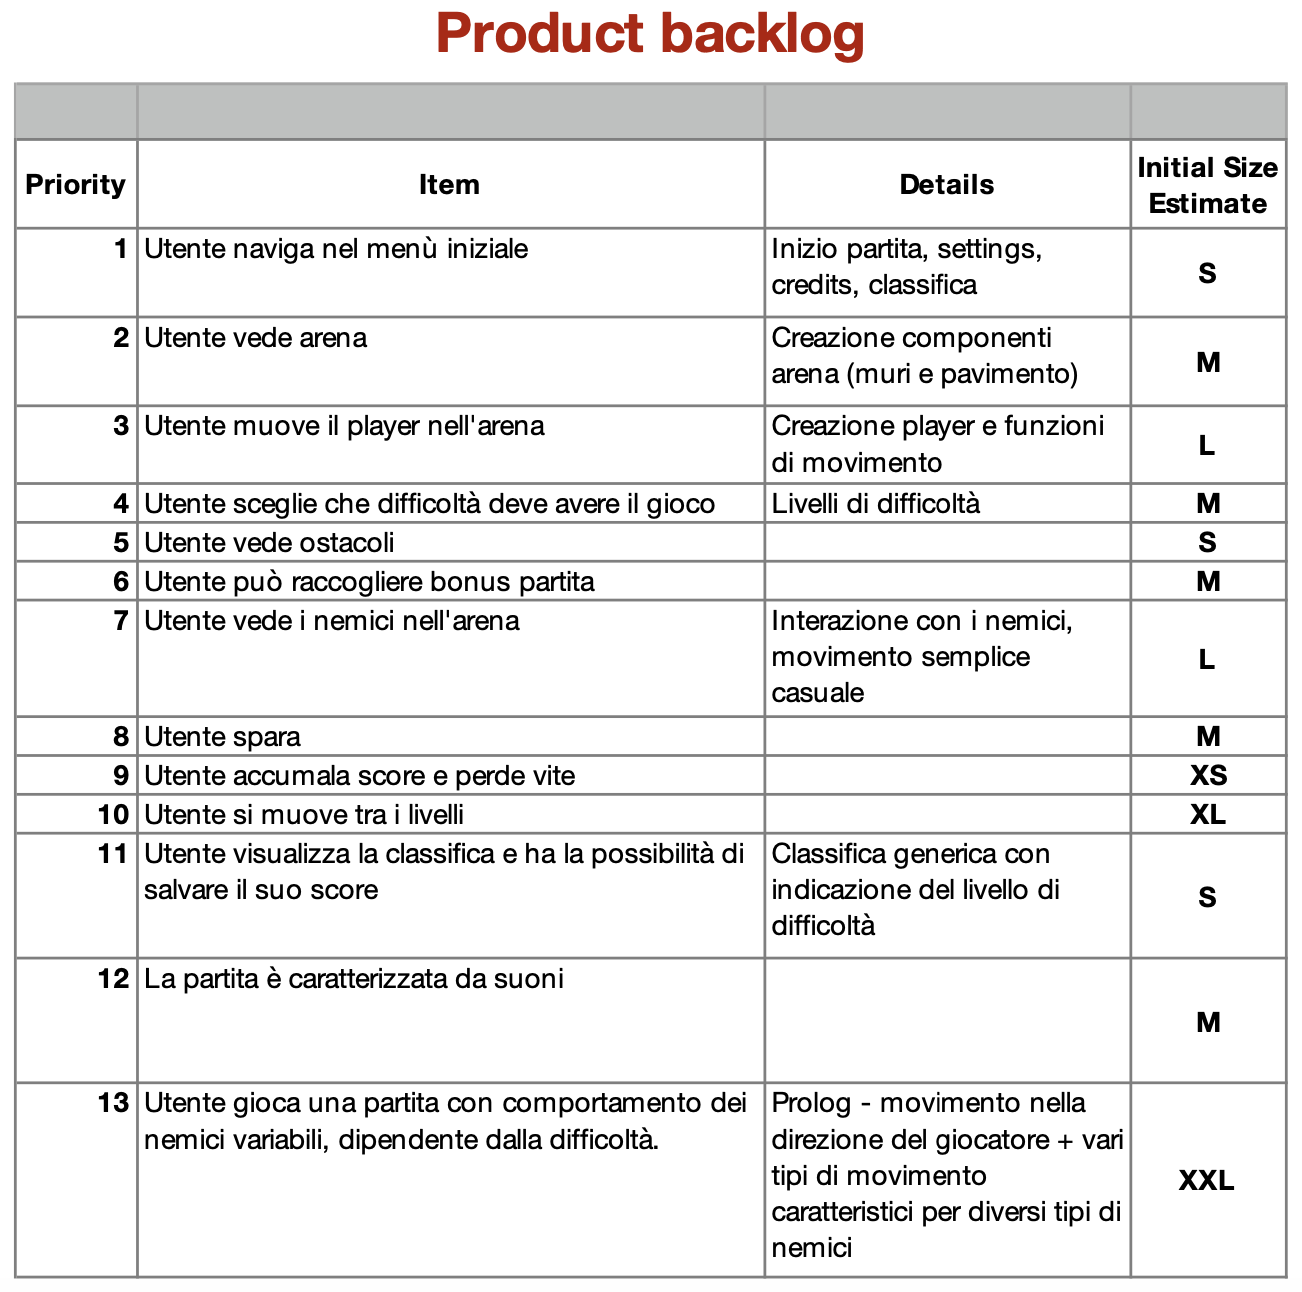
\includegraphics[width=13cm]{res/backlog.png}
  \caption{Product Backlog}
  \label{notifyAction}
\end{figure}
        \section{Strumenti utilizzati}\label{sec:tools}
            \subsection{Versioning}\label{subsec:versioning}
Il sistema di \textit{versioning} ha ricorperto un ruolo centrale nella realizzazione del progetto e per tale scopo abbiamo scelto di utilizzare \textbf{Git}.
Per quanto riguarda l'hosting del repository abbiamo optato per la piattaforma \textbf{GitHub}.

Il flusso di lavoro è stato definito secondo le linee guida del metodo di branching \textbf{git-flow}:
\begin{itemize}
	\item Il branch \textit{master} contiene il codice relativo a ciascuna release.
	\item Il branch \textit{development} ospita il codice realizzato durante uno sprint. Tale codice è testato e stabile, ma non ancora giudicato completamente utilizzabile.
	\item I vari branch \textit{task-*} corrispondono a ciascun task individuato durante i vari sprint. Tale codice è in fase di implementazione e può contenere codice non completamente funzionante, in quanto ancora in sviluppo.
	\item non sono stati necessari branch di \textit{hotfix}.
\end{itemize}

\subsection{Dependency management \& buildscript}\label{subsec:build}

Per la gestione delle dipendenze, quali ad esempio librerie o plugin, e la compilazione del codice, come strumento di automazione dello sviluppo si è utilizzato \textbf{sbt}.
In particolare, sono stati scritti buildscript per automatizzare:

\begin{itemize}
    \item la gestione delle \textit{dipendenze} provenienti da repository Maven;
    \item il processo di \textit{testing} tramite ScalaTest e controllo di \textit{qualità del codice} tramite Scalastyle;
    \item la gestione delle dipendenze dei vari moduli di \textit{JavaFX} per le varie versione di Java.
    \item generazione dei \textit{Jar} eseguibili.
\end{itemize}

\subsection{Continuous Integration}\label{subsec:ci}

Per la verifica del codice prodotto e dei reativi test si è optato per \textit{Travis CI}.
Questo servizio offre la possibilità di registrare un web-hook al repository GitHub su cui è istanziato il progetto, così da provocare l'esecuzione di Travis CI ad ogni commit effettuato sul repository.
La configurazione di Travis è stata definita utilizzando il formato YAML e in particolare sono stati specificati:
\begin{itemize}
	\item il linguaggio (Scala);
	\item la versione di Scala;
	\item la JDK da utilizzare.
\end{itemize}

	\clearpage
	
	\chapter{Analisi del dominio}\label{ch:analisi}
		\section{Descrizione del gioco}\label{sec:gamedescription}
		Il progetto consiste nello sviluppo di un gioco di tipo Battle Arena con grafica 2D a visuale fissa. Il giocatore interpreta un personaggio che si muove all'interno di una mappa generata casualmente, sconfiggendo nemici e completando livelli.

Il giocatore si sposta da una stanza di dimensioni fisse ad un'altra, che rappresentano i diversi livelli del gioco.
Una stanza può contenere un numero arbitrario di nemici, oggetti collezionabili e ostacoli; sconfiggere tutti i nemici garantisce l'accesso al livello successivo. Solo una stanza è visibile a schermo in un dato momento.

L'obiettivo del gioco potrebbe essere quello di raggiungere una stanza contenente un oggetto speciale che determina la fine della partita, o, in alternativa, il completamento di un certo numero di stanze.
Nel primo caso, anche la probabilità di trovare l'oggetto speciale è casuale, ma comunque dipendente da alcune condizioni di gioco (come, ad esempio, il raggiungimento di una soglia di punteggio).
Tuttavia, il gioco potrebbe essere giocato in una modalità che ha come scopo la sopravvivenza, solo per ottenere un punteggio personale più alto, che viene mantenuto salvato e mostrato nella sezione della classifica del menu.
La natura casuale del gioco implica una curva di difficoltà facilmente variabile, facendo dipendere il gameplay anche dalla fortuna, che può renderlo divertente ma a volte anche impegnativo.

L'arma principale a disposizione del giocatore sono proiettili (pomodori) da lanciare ai nemici; gli oggetti collezionabili garantiscono un bonus di punteggio o di vita.

Il gioco consente di registrare diversi profili utente per salvare le statistiche di gioco e confrontarle in una classifica.

    \clearpage

    \chapter{Requisiti}\label{ch:requirements}
        Durante la fase iniziale del progetto ci siamo suddivisi i task da svolgere per sprint cercando di mantenere coerenza con i vari ambiti.
D'altro canto, per poterci aiutare a vicenda è capitato un po' per tutti di andare a toccare il codice di altri componenti, finendo così ad avere un codice nel quale hanno messo le mani un po' tutti.
Inoltre, per i task più complessi, si è deciso di optare per la tecnica di \textit{pair programming}.
        \section{Requisiti di business}\label{sec:requirements:businee}
            Sono stati individuati i seguenti requisiti necessari per la realizzazione del progetto:
\begin{itemize}
	\item possibilità di avviare una partita tramite un menu di gioco
	\item possibilità di comandare un personaggio all'interno di una mappa di gioco
	\item possibilità di salvare i dati del giocatore
\end{itemize}
        \section{Requisiti utente}\label{sec:requirements:user}
            Sono stati poi individuati i requisiti che rappresentano ciò che l'utente deve poter fare con l'applicazione.
Un utente potrà:
\begin{itemize}
	\item scegliere la difficoltà di gioco;
	\item avviare una partita attraverso un menu, che dovrà contenere almeno le seguenti voci:
	\begin{itemize}
	    \item iniziare una nuova partita;
	    \item visualizzare i punteggi;
	    \item modificare le impostazioni.
	\end{itemize}
	\item sconfiggere nemici, che devono essere:
	\begin{itemize}
	    \item dotati di un movimento indipendente;
	    \item capaci di danneggiare il giocatore;
	    \item dipendenti dalla difficoltà;
	    \item necessari per il completamento del livello.
	\end{itemize}
	\item raccogliere oggetti ed evitare ostacoli;
	\item accumulare un punteggio quando progredisce nel gioco, che si ottiene in caso di:
	\begin{itemize}
	    \item uccisione di un nemico;
	    \item raccoglimento di un oggetto collezionabile.
	\end{itemize}
	\item salvare automaticamente il proprio punteggio;
	\item visualizzare la classifica di tutti i profili registrati.
\end{itemize}
        \section{Requisiti funzionali}\label{sec:requirements:functional}
            In questa sezione si andranno ad elencare i vari requisisti funzionali che sono quelle funzionalità specifiche che l'applicazione implementa:
\begin{itemize}
	\item possibilità di giocare una partita ad un gioco battle arena in locale;
	\item sviluppare un'interfaccia di gioco con grafica 2D fissa;
	\item gestire la logica e il coordinamento delle partite: gestione del movimento e delle vite del giocatore e dei nemici, gestione dei bonus e gestione del punteggio;
	\item possibilità di passare da un livello di gioco ad un altro;
	\item gestire opportunatamente le varie difficoltà di gioco;
	\item possibilità di salvare e visualizzare la classifica globale dei punteggi di gioco.
\end{itemize}
\comment{            
            \subsection{Regole di gioco}\label{subsec:requirements:game}
                \input{3-requisiti/rules.tex} 
            \subsection{Ranked Mode}\label{subsec:requirements:ranked}
                \input{3-requisiti/ranked.tex}
            \subsection[Interfaccia utente]{Interfaccia grafica per l'utente}\label{subsec:requirements:gui}
                \input{3-requisiti/ui.tex}
                }
        \section{Requisiti non funzionali}\label{sec:requirements:notfunctional}
           	In questa sezione, invece, si andranno ad elencare quei requisiti che fanno riferimento ai vincoli e alla qualità del sistema.
\begin{itemize}
	\item \textit{Modularità}: il sistema dovrà essere composto da moduli separati ed indipendenti in modo tale da facilitare la resistenza ai guasti e il testing.
	\item \textit{Estensibilità}: il sistema dovrà essere progettato e implementato in modo tale da facilitare l'aggiunta di nuove funzionalità o la modifica quelle già esistenti.
	\item \textit{Consistenza}: il sistema dovrà mantenere lo stato del gioco coerente con le varie impostazioni immesse dall'utente e con ciò che accade durante la partita.
	\item \textit{Reattività}: il sistema fornirà risposte con bassa latenza alle varie interazioni dell'utente.
\end{itemize}
        \section{Requisiti implementativi}\label{sec:requirements:implementative}
            I requisiti implementativi riguardano quei requisiti che assicurano la qualità di un software.
Il codice creato dovrà:
\begin{itemize}
	\item utilizzare un paradigma di tipo funzionale;
	\item facilitare la scalabilità usando strutture dati immutabili;
	\item non avere side-effect;
	\item dovrà soddisfare dei requisiti di stile;
	\item dovrà soddisfare dei test.
\end{itemize}

    \clearpage

    \chapter{Design architetturale}\label{ch:design}
        
        \section[Architettura]{Architettura complessiva}\label{sec:architecture}
        Per lo sviluppo del gioco si è scelto di utilizzare il pattern MVC in quanto si vuole avere una separazione pulita tra la parte logica e la parte di visualizzazione. In questo modo si lascia aperta la possibilità di avere diversi tipi di interfaccia grafica.

Inoltre si è scelto di utilizzare un event-loop per gestire la ricezione di input utente, l'update della parte logica e l'update della parte di interfaccia grafica. 

Di seguito è riportato un diagramma che illustra le classi principali per la comunicazione tra Model-View-Controller.

\begin{figure}[H]
  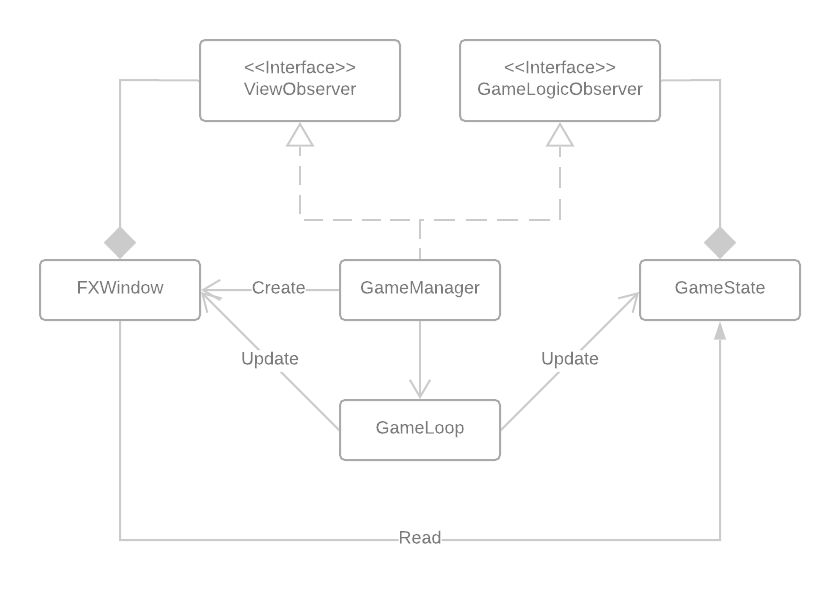
\includegraphics[width=15cm]{report/res/MVC_Diagram.png}
  \caption{Utilizzo pattern MVC}
\end{figure}
            \subsection{Model}\label{subsec:architecture:model}
                Contiene la logica di gioco. 

\begin{itemize}
    \item \textbf{GameState}: rappresenta il mezzo con cui, dall'esterno, ci si può interfacciare con la logica di gioco. Fornisce una serie di funzionalità per gestire la partita, come ad esempio far partire il gioco, chiamare il prossimo step, creare un nuovo livello e gestire i record. All'interno di \textit{GameState} si trova un'istanza della classe \textit{Arena} che rappresenta la mappa di gioco contenente le entità e le varie relazione tra esse.
    
    \item \textbf{MapGenerator}: utilizzato al fine di posizionare nell'ambiente di gioco le proprie entità di partenza come gli ostacoli, i nemici e gli oggetti collezionabili.
    
    \item \textbf{Entity}: come riportato in figura \ref{model}, tutti gli elementi del gioco estendono da questa interfaccia generica. Inoltre  all'entità di base, grazie all'ereditarietà multipla fornita da Scala, si possono decorare le entità con diverse caratteristiche come ad esempio la possibilità di muoversi o di avere una vita. 
\end{itemize}

\begin{figure}[H]
  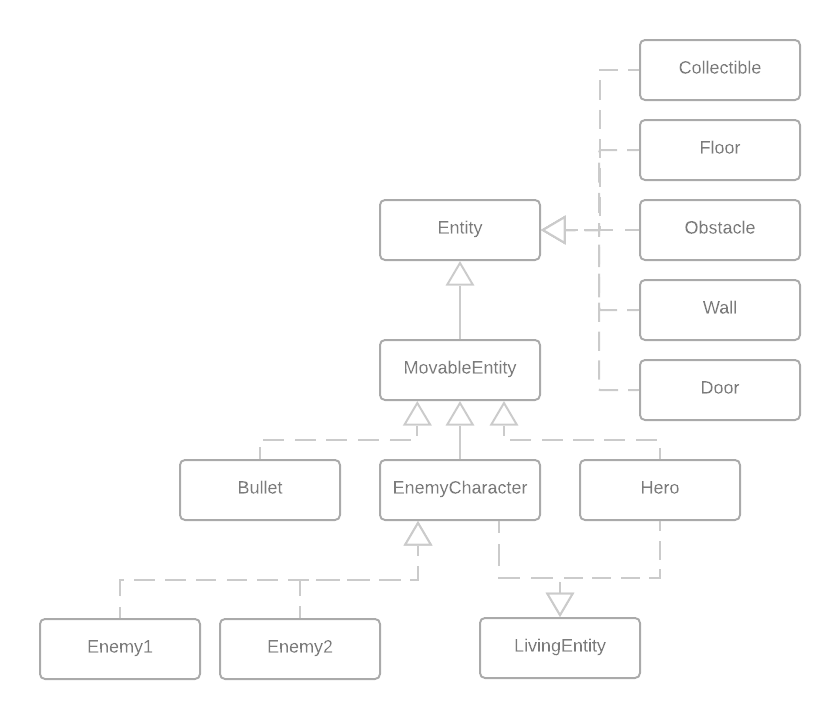
\includegraphics[width=15cm]{report/res/GAMELOGIC_Diagram.png}
  \caption{Organizzazione della logica di gioco}
  \label{model}
\end{figure}
             \subsection{View}\label{subsec:architecture:view}
                Ha il compito di mostrare i dati forniti dal \textit{GameLogic}. 
La \textit{GameView} è costituita fondamentalmente da due parti:

\begin{itemize}
    \item Menù di gioco che comprende:
    \begin{itemize}
        \item Credits
        \item Ranking: classifica globale dell'utente
        \item Settings: da la possibilità di settare il nome del player e la difficoltà di gioco
    \end{itemize}
    \item Arena di gioco: Aggiornata dal \textit{GameManager} ad ogni step. Mantiene una serie di \textit{Map} che rappresentano i vari elementi che devono essere disegnati e spostati ad ogni step. La collezione mappa l'id dell'elemento alla propria \textit{ImageView}. Ad ogni update, tramite le \textit{case class} di supporto descritte in figura \ref{view}, si controlla se gli elementi hanno subito variazioni dall'update precedente, in caso affermativo vengono ridisegnate nella posizione corretta o eliminate.
    Mantenendo questa serie di \textit{Map} si evita di svuotare e ripopolare l'arena di gioco ad ogni step. In questo modo non si rischia di sovraccaricare il \textit{JavaFX Application Thread}.
\end{itemize}

\begin{figure}[H]
  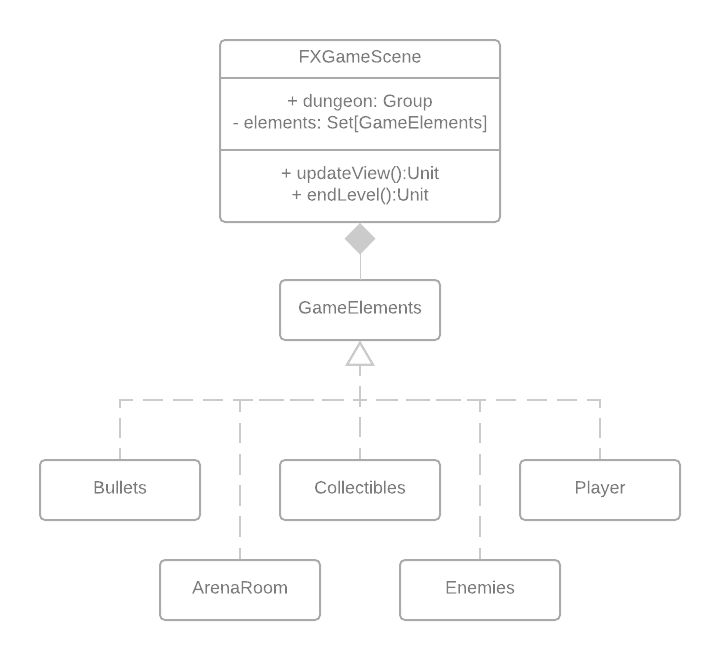
\includegraphics[width=13cm]{report/res/VIEW_Diagram.png}
  \caption{Organizzazione dell'arena di gioco}
  \label{view}
\end{figure}
             \subsection{Controller}\label{subsec:architecture:controller}
                
\subsubsection{GameManager} Principale elemento relativo al controller ed ha varie funzionalità. Una di queste è \textit{initializeGame}. per l'inizializzazione del gioco: questo metodo permette di inizializzare la parte di \textit{GameView}, inoltre permette il caricamento di tutte le sprites utilizzate successivamente nella partita.
    
\textit{GameManager} rappresenta un ponte tra la \textit{GameView} e il \textit{GameLogic}, in quanto ascolta gli eventi compiuti dall'utente lato \textit{GameView} e li comunica al \textit{GameLogic}. 
    Per osservare gli eventi della view il \textit{GameManager} implementa il \textit{ViewObserver}, che verrà approfondito in un'altra sezione.
    inoltre il \textit{GameManager} implementa il \textit{GameLogicObserver}, si è scelto di usare il pattern observer per permettere al \textit{GameLogic} di notificare ogni qual volta viene eseguita un azione. Questo viene poi sfruttato dal GameManager per la riproduzione dei suoni.
    
    \subsubsection{GameLoop} Si è scelto di utilizzare un approccio ad event-loop single-thread per gestire le dinamiche di gioco. In accordo con i colleghi, questo approccio è stato scelto poichè si adatta bene al tipo di gioco sviluppato: il \textit{GameLoop} ha in particolare due task fondamentali da svolgere in sequenza, ovvero deve aggiornare la parte di \textit{GameLogic} e successivamente aggiornare la parte di \textit{GameView}. Inoltre l'approccio a event-loop, essendo in esecuzione su un singolo thread e processando un task alla volta, risulta essere thread safe.
    Quindi questa classe è incaricata di implementare l'Event-loop: all'avvio della partita il \textit{GameManager} fa partire un thread separato sul quale viene lanciato un event-loop incaricato di aggiornare la parte view ed, ad ogni ciclo, far compiere uno step alla parte logica.
    Per gestire gli eventi generati dall'utente vengono utilizzate due queue che tengono traccia degli spari e dei movimenti compiuti dall'utente e non ancora processati dall'event-loop. Gli eventi vengono poi recuperati ad ogni step come riportato in figura \ref{checknewMovement}, e passati al \textit{GameState} che li elaborerà. 
    
    \begin{figure}[H]
    \centering
      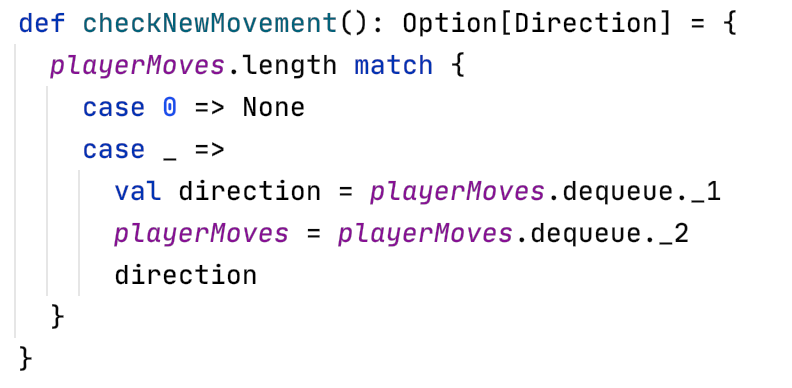
\includegraphics[width=10cm]{res/checkNewMovement.png}
      \caption{Recupera un movimento notificato}
      \label{checknewMovement}
    \end{figure}
    
    Una struttura generale della gestione degli eventi è riportata in figura \ref{gameLoop}: \textit{FXGameScene} rappresenta l'emitter degli eventi, che vengono poi, tramite \textit{GameManager}, salvati in due queue da cui il \textit{GameLoop} recupererà i singoli eventi e li darà in pasto al \textit{GameState}.
    
    \begin{figure}[H]
    \centering
      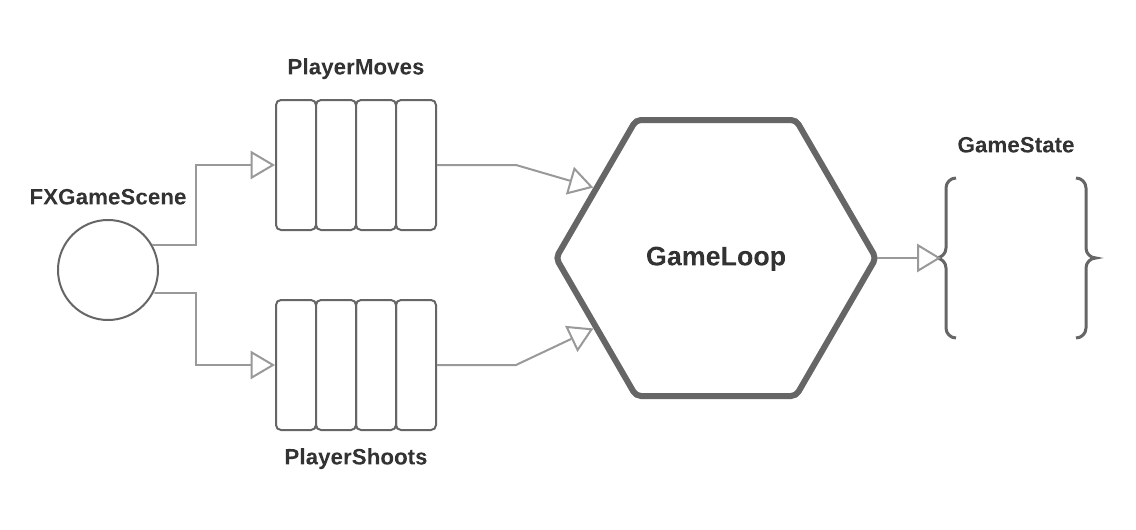
\includegraphics[width=14cm]{res/event_loop_diagram.png}
      \caption{Struttura gestione eventi}
      \label{gameLoop}
    \end{figure}
    
    \subsubsection{ImageLoader} Come accennato in precedenza, esso permette, all'apertura dell'applicazione, di caricare tutte le sprites utilizzate successivamente, in modo da limitare le letture da file durante l'esecuzione del gioco; questa operazione è fatta sfruttanto il meccanismo delle Future, quindi al suo completamento verrà visualizzata la finestra dell'applicazione. 
    Durante l'esecuzione del gioco invece permette alla \textit{GameView} di recuperare le \textit{Image} di cui ha bisogno.
    
    \subsubsection{SoundLoader} Gestisce la riproduzione dei suoni all'interno del gioco. Quando viene richiesta la riproduzione di un suono, viene generata una nuova \textit{Future} che creerà lo stream e quindi il clip per poi riprodurlo.


    \clearpage

    \chapter{Design di dettaglio}\label{ch:details}
        Durante la fase iniziale del progetto ci siamo suddivisi i task da svolgere per sprint cercando di mantenere coerenza con i vari ambiti.
D'altro canto, per poterci aiutare a vicenda è capitato un po' per tutti di andare a toccare il codice di altri componenti, finendo così ad avere un codice nel quale hanno messo le mani un po' tutti.
Inoltre, per i task più complessi, si è deciso di optare per la tecnica di \textit{pair programming}.
        \section{Organizzazione del codice}\label{sec:organizations}
         Partendo dal design architetturale, il codice è stato diviso nei tre package \textit{gamelogic}, \textit{gamemanager} e \textit{gameview} per rispecchiare il pattern MVC; un quarto package chiamato \textit{utilities} contiene invece funzionalità utili a tutti e tre. Di seguito la descrizione dei principali elementi di ogni package e delle loro funzionalità.
         \section{Pattern utilizzati}\label{sec:pattern}
          Durante l'intero progetto di sviluppo sono stati inclusi diversi pattern e aspetti di degin avanzato.

Primo fra tutti il \textbf{Singleton} che è stato ampiamente utilizzato, in quanto Scala tutti gli object sono Singleton.
Poi il pattern \textbf{Observer}, si vedano le classi \textit{ViewObserver} e \textit{GameLogicObserver}, il pattern \textbf{Builder} come la classe \textit{StaticArena} per la generazione di \textit{Arena} in maniera deterministica.
\`E stato utilizzato, inoltre, il pattern \textbf{Decorator}, vedasi \textit{LivingEntity}.
        \section{Scelte rilevanti}\label{sec:choices}
           Prima e durante la fase di sviluppo è stato necessario valutare delle scelte di implementazione, principalmente per cercare di sfruttare al meglio le caratteristiche di Scala, in modo da scrivere del codice intuitivo, compatto e scalabile, cercando anche di trarre il meglio dal paradigma funzionale e di garantire il più possibile immutablità e assenza di side-effect; un altro motivo di scelta principale ha riguardato anche la pesantezza del codice, avendo a che fare con un'applicazione particolarmente dinamica e reattiva. Di seguito sono riportate le scelte più significative che sono state adottate in fase di sviluppo:

\begin{itemize}
    \item \textbf{Case class}: Una scelta fondamentale, in quanto legata all'immutabilità del codice, ha riguardato l'utilizzo delle case class, in particolare per le entità. Queste sono caratterizzate da una posizione che per molte di esse cambia ad ogni step, ma volendo mantenerne lo stato immutabile, si è puntato a dichiararle come case class, in modo da poterle facilmente istanziare nuovamente a seguito di una modifica dello stato, nonchè per la facilità d'uso all'interno dei costrutti match-case. La gestione dello stato delle entità in questo modo è stata anche oggetto di refactoring durante lo sviluppo.
    
    Altra questione non meno importante riguarda la dichiarazione delle strutture dati nella classe \textit{Arena} (ma anche nel resto del programma), che possono potenzialmente rappresentare il collo di bottiglia per la velocità di esecuzione complessiva dell'applicazione. Seguendo la stessa logica utilizzata per le case class, sono sempre state usate strutture immutabili, dichiarate come var per garantirne la sostituzione in seguito ad un loro aggiornamento. L'immutabilità in questo caso assicura la coerenza nello stato del model.

    \item \textbf{GameLoop}: Il loop di controllo è stato oggetto di rifattorizzazione per quanto riguarda la struttura del ciclo e l'implementazione del suo thread. Il ciclo inizialmente seguiva una logica ricorsiva ed è stato poi convertito in un più semplice while-loop, per motivi meramente legati alla velocità di esecuzione, essendo un punto cruciale per il flusso logico del programma; la classe, invece, è passata dall'estendere \textit{Thread} all'implementare \textit{Runnable}, volendo avere una concorrenza basata sui task.
\end{itemize}
           
    \clearpage

    \chapter{Implementazione}\label{ch:implementation}
        
        \section{Lorenzo Chiana}\label{sec:chiana}
            \subsection{Gamelogic}
La parte di progettazione dei vari componenti di base non è spettata a me, ma ho contribuito lo stesso, dal secondo sprint in poi, con diverse modifiche e rifattorizzazioni a classi e metodi del model, a volte anche in pair programming con Meshua Galassi (come per il task "Creazione nemici lato model" nel terzo sprint).
Inoltre, contributo significativo all'interno della parte di model sono stati diversi bugfixing nel corso degli sprint.
Le varie classi che ho toccato maggiormente sono: \textit{Arena}, \textit{Enemy}, \textit{MapGenerator}, \textit{MovableEntity}, \textit{Obstacle}, \textit{ObstacleTypes} e \textit{Player}.

\subsubsection{Arena}
In Arena mi sono occuppato dei vari metodi che vanno a controllare se un punto contiene una certa entità come \textit{containsCollectible()}, \textit{containsObstacle()} e così via.
Inoltre in vari task sono andato a toccare e rifattorizzare il metodo \textit{checkMovement()} per introdurre la collezione dei bonus e controllo della collisione con nemici e conseguente pardita di vita dell'eroe.

\subsubsection{Enemy e MovableEntity}
Durante il terzo sprint mi sono occupato insieme a Meshua Galassi della generazione dei nemici, in particolare mi sono occupato della rifattorizzazione del vecchio metodo \textit{canMove()}.

\subsubsection{MapGenerator}
Mi sono occupato della rifattorizzazione dei metodi \textit{generateEnemies()}, \textit{generateCollectibles()} e \textit{generateObstacles()}.

\subsubsection{Obstacle e ObstacleTypes}
Inizialmente gli ostacoli non avevano un tipo e non era possibile distirguerli per associargli sprite diverse.
Per ovviare a questa problematica ho implementato la possibilità di avere tre diverse tipologie di ostacoli in maniera casuale rifattorizzando il tutto.

\subsubsection{Player}
Rifattorizzato introducendo la possibilità di avere un record personale.

\subsubsection{Dopo le varie rifattorizzazioni}
Dopo varie rifattorizzazioni susseguite nei vari sprint del mio contributo più significativo rimane:
\begin{itemize}
	\item la rifattorizzazione ai metodi \textit{generateEnemies()}, \textit{generateCollectibles()} e \textit{generateObstacles()} all'interno di \textit{MapGenerator};
	\item la gestione dei record del giocatore ed aggiornamento della classifica in \textit{Player} e \textit{GameState};
	\item la creazione e rifattorizzazione di metodi come \textit{containsCollectible()}, \textit{containsObstacle()}, \textit{containsWall()}, \textit{containsEnemy()} e \textit{containsBullet()} di \textit{Arena};
	\item la creazione di \textit{ObstacleTypes}.
\end{itemize}


\subsection{Gameview}
Durante il primo sprint mi sono occupato della progettazione e realizzazione dei mockup del menù di gioco, andando a creare le principali voci del menù che, ancora nell'ultima versione, sono presenti, quali "\textit{Settings}" e "\textit{Credits}".
Inoltre, per quanto riguarda l'interfaccia di gioco, ho realizzato un prima versione base dell'arena di gioco accessibile attraverso la voce del menù "\textit{Start game}".
Dal quarto sprint ho introdotto anche la voce "\textit{Player rankings}" con relativa scena.
Le varie interfacce dei singoli componenti della view sono stati progettati e realizzati ponendo attenzione a renderli indipendenti dalla piattaforma anche grazie all'utilizzo di file \textit{CSS} e \textit{FXML}.
Quest'ultima tipologia di file è stata prodotta grazie all'utilizzo del tool \textit{Scene Builder}.

Inoltre mi sono occupato della generazione grafica dell'arena, andando a creare le sprite delle varie entità dapprima in modo statico e poi, dal secondo sprint, in modo dinamico a seconda delle informazioni contenute nel model.
In un secondo momento questa generazione grafica è stata rifattorizzata da Giada Gibertoni, andando a snellire la classe \textit{FXGameScene} e portandola alla struttura che ha oggi \ref{view}.

\subsubsection{Scelta della libreria}

Prima della progettazione e implementazione dell'interfaccia mi sono concentrato insieme alla collega Giada Gibertoni sulla ricerca di una libreria grafica da utilizzare.
Il primo risultato di questa ricerca è ricaduto su \textit{ScalaFX} che ricalca lo stile di \textit{JavaFX} però in termini molto più Scala-like.
D'altro canto ci si è accorti quasi subito che è molto scarna di esempi pratici e per questo motivo alla fine abbiamo abbandonato l'idea di utilizzare questa libreria.
La ricerca è proseguita su altre librerie tutte scartate o per il medesimo motivo o perché non davano la possibilità di definire l'interfaccia grafica tramite file esterni, limitando il tutto a dover disegnare la GUI tramite classi.
Alla fine si è optato per JavaFX, soprattutto perché offre tanti esempi reperibili online grazie ad una community molto attiva e anche perché offre un'integrazione con file esterni come FXML.

\subsubsection{Finestra generica e implementazione in JavaFX}

Data questa incertezza iniziale sulla scelta della libreria grafica, sono andato a creare una finestra generica grazie alla quale un eventuale futuro cambio di libreria non avrebbe portato comportamenti inattesi nel comportamento di base della finestra.
Una volta definite le funzionalità di base nell'interfaccia \textit{Window}, questa sarà implementata da \textit{FXWindow} che va a creare una finestra conforme agli standard di JavaFX.

\begin{figure}[H]
  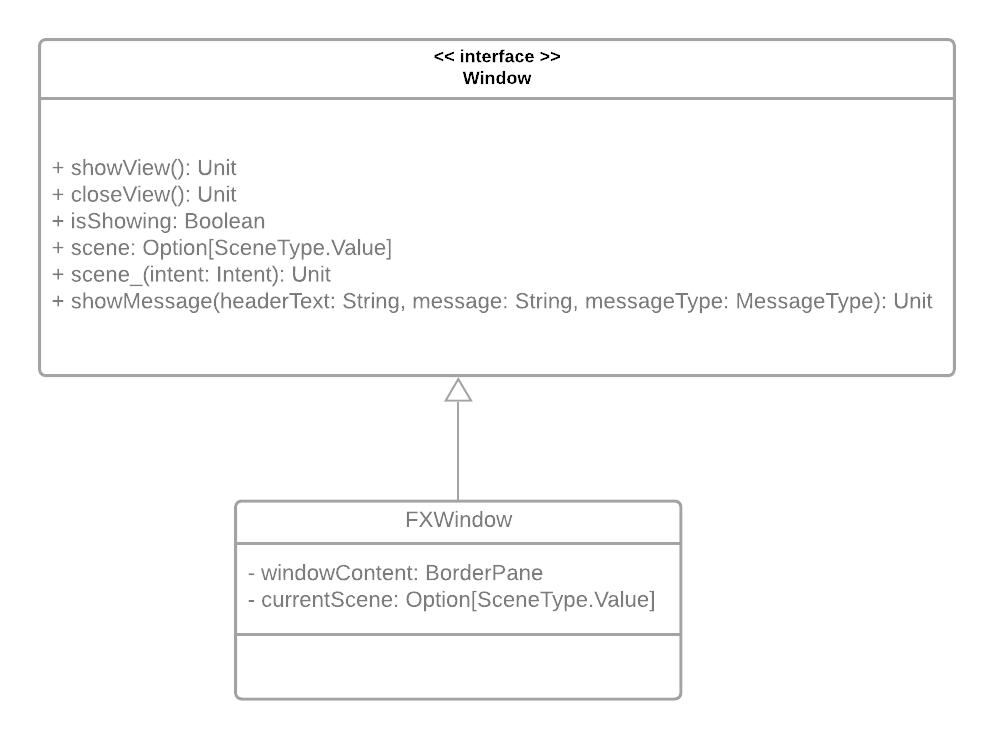
\includegraphics[width=15cm]{res/6-implementazione/chiana/UML_Window.png}
  \caption{Interfaccia Window e FXWindow che la implementa.}
  \label{windowClass}
\end{figure}

\subsubsection{Navigazione e scene}
La navigazione tra le schermate viene permesso grazie al metodo \textit{scene\textunderscore()} che va a creare la nuova scena e a notificare all'observer (\textit{GameManager}) che deve cambiare la scena con la nuova.
La decisione su che scena creare viene presa sul tipo di scena (\textit{SceneType}), un'\textit{Enumeration} passata come parametro all'\textit{Intent} (classe che rappresenta l'intento di cambiare la scena corrente con un'altra).

\subsubsection{Arena di gioco}
Mi sono inoltre occupato della creazione dell'interfaccia di gioco, andando a creare visualmente l'arena che il giocatore vedrà mentre gioca, all'interno di \textit{FXGameScene}.
Qui ogni punto dell'arena logica viene tradotto in una piastrella alla quale viene assegnata una certa sprite a seconda della tipologia dell'entità che è presente su tale punto (metodo \textit{createArena()}).
Queste piastrelle vengono regolarmente aggiornate ed allineate con la parte logica del programma tramite il metodo \textit{nextStep()} di \textit{GameLoop}.
La realizzazione di FXGameScene è stata incrementale durante tutto lo sviluppo del gioco, tant'è che ha subito diverse modifiche e aggiunte da diversi componenti del gruppo.

\subsection{Gamemanager}
La parte di gamemanager, come per la parte di gamelogic, la sono andato a toccare diverse volte, ma solo con piccole modifiche e rifattorizzazioni.
I contributi più significativi che ho dato in questa parte del progetto si possono suddividere in: \textit{PreferencesHandler} e \textit{caricamento e salvataggio della classifica di gioco}.

\subsubsection{PreferencesHandler}
Viene utilizzata per salvare le preferenze dell'utente come il nome e la difficoltà di gioco attraverso l'uso di \textit{Java Preferences API}.
Il salvataggio e la serializzazione di queste impostazioni vengono fatte attraverso l'estensione \textit{lift-json-ext} che verrà poi utilizzata anche per salvare la classifica di gioco.

\subsubsection{Classifica di gioco}
La classifica di gioco viene salvata in un file JSON tramite la \textit{PrintWriter} di \textit{java.io} con la seguente struttura: \ref{json}

\begin{figure}[H]
  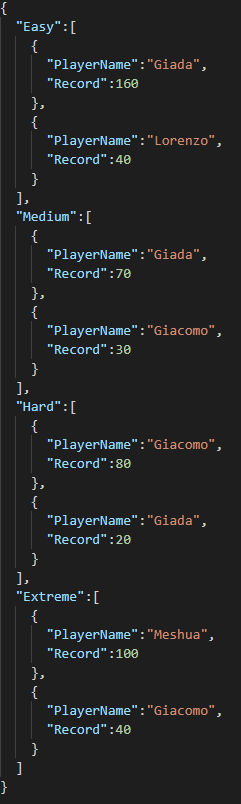
\includegraphics[width=5cm]{res/6-implementazione/chiana/json.png}
  \caption{Struttura del file rank.json}
  \label{json}
\end{figure}

Questo file viene letto tramite il metodo \textit{loadPlayerRankings()} di \textit{GameManager} andando a creare una mappa che come chiave presenta il nome della difficoltà e come valore un'altra mappa che, a sua volta, come chiave ha il nome del giocatore e come valore il suo record.
Questa mappa viene salvata in \textit{GameState} (all'interno di gamelogic) e aggiornata dinamicamente durante il gioco.
Alla fine di ogni partita la mappa viene salvata nel file JSON attraverso il metodo \textit{savePlayerRankings()}.

Durante il task relativo alla creazione della classifica ho scelto di adottare la libreria lift-json del framework Lift, perché una delle più utilizzate e consigliate per i progetti Scala.

\subsection{Utilities}
Nei vari sprint a seconda dell'esigenza sono andato a creare:
\begin{itemize}
	\item Animations: utilizzata per creare un animazione di fade-in o fade-out tra le varie scene;
	\item Intent: classe che rappresenta l'intento di cambiare la scena corrente con un'altra;
	\item MessageTypes: un sailed trait che rappresenta i vari tipi di messaggi di una finestra di dialogo;
	\item ViewLoader: permette il caricamento, e quindi l'utilizzo, di layout in formato \textit{.fxml};
	\item WindowSize: contiene le dimensioni della finestra del menù principale e di quella di gioco.
		
\end{itemize}

\subsection{Test}
Per quanto riguarda la parte di testing mi sono occupato di andare a testare le classi \textit{Player}, \textit{Hero}, \textit{Enemy} e \textit{Bullet} con \textit{AnyFlatSpec} come tipologia di sintassi.

Per ogni entità sono andato a testare le caratteristiche principali come ad esempio la direzione del movimento, le collisioni, eventuali decrementi o incrementi di vita o di punteggio e così via.
L'unico inconveniente di questo approccio era dato dalla casualità di creazione dell'arena di gioco che poteva far fallire alcuni test come, ad esempio, testare il movimento in una certa direzione.
In questo caso si poteva presentare il caso in cui, nel punto in cui si doveva muovere l'entità, era presente un'altra entità finendo per colliderci e risultando di consenguenza non essersi mossa.
Per ovviare a questo problema ho optato nella creazione di una classe builder \textit{StaticArena} nella quale l'arena generata casualmente viene svuotata e impostata con delle entità in determinati punti passatagli come parametri, permettendo così di creare una scena ad hoc per il test da eseguire.

\subsection{Environment}
Dell'ambiente di sviluppo mi sono occupato di impostare in sbt i plugin \textit{ScalaStyle}, per il controllo dello stile, e \textit{sbt-assembly}, per il deploy del file jar.
Inoltre mi sono occupato della configurazione di Travis CI, andando ad impostare la versione di Scala, la directory del progetto, e la versione della JDK da utilizzare.

    
        %\clearpage
        
        \section{Meshua Galassi}\label{sec:galassi}
            \input{6-implementazione/galassi/galassi.tex}

        \clearpage
    
        \section{Giada Gibertoni}\label{sec:gibertoni}
            La maggior parte del mio lavoro si è concentrata sull'implementazione della parte \textit{GameView} e della parte \textit{GameManager}, ho aiutato anche i miei compagni nella parte relativa alla \textit{GameLogic}. Inoltre ho partecipato, insieme ai miei colleghi, alla risoluzione di vari bug e alla rifattorizzazione del codice.
Infine, insieme a Lorenzo Chiana, ho impostato il file \textit{build.sbt}.


        
        %\clearpage
        
        \section{Giacomo Pasini}\label{sec:pasini}
            \input{6-implementazione/pasini/pasini.tex}

    \clearpage

    \chapter{Retrospettiva e commenti finali}\label{ch:retrospective}
        Analizzando il nostro percorso di sviluppo, ci siamo accorti che si potrebbero introdurre migliorie sia per quanto riguarda la parte implementativa che per quanto riguarda quella organizzativa.

\subsubsection{Punto di vista organizzativo}
Nonostante abbiamo fatto una buona pianificazione, seguendo la metodologia scrum ed utilizzando Trello, qualche volta non sono state rispettate le linee guida previste per la sprint. Ovvero, a volte non sono state rispettate le urgenze indicate nei task in quanto venivano svolti prima task con un grado di urgenza inferiore.

Inoltre, sarebbe stato più appropriato utilizzare una metodologia git-flow basata su fork/pull request poichè, in questo modo si sarebbe introdotto un ulteriore controllo sulla qualità del codice caricato all'interno del repository.

\subsubsection{Punto di vista implementativo}
Avendo inizialmente sottovalutato la complessità dei calcoli presenti all'interno del gamelogic, è stato scelto un approccio di tipo single thread. Guardando lo stato finale del progetto, la complessità del gameLogic è salita, quindi sarebbe stato meglio se le computazioni al suo interno fossero state sviluppate concorretemente. In questo modo, si sarebbero evitati, probabilmente, anche i problemi nati con l'introduzione del codice Prolog.


        
\end{document}
